Para una correcta implementaci�n del m�todo HIL, se debe tener un emulador para la planta, que fue seleccionado en el cap�tulo \ref{CAP:tecni}, y esto con el objetivo de hacer pruebas a un controlador real que es representado dentro del dispositivo microcontrolador. 


\section{Posibles dispositivos para dise�ar el controlador}

\subsection{Arduino Ethernet}


%\begin{figure}[H]
%	\centering
%	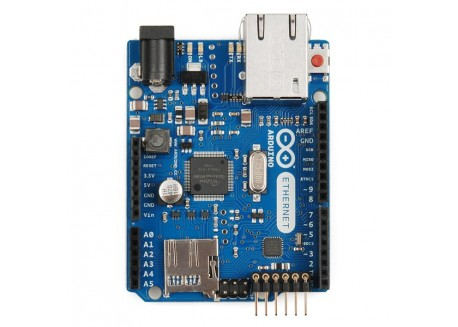
\includegraphics[width=0.7\linewidth]{img/arduinoethernet}
%	\caption{Arduino Ethernet}{Fuente: {\cite{arduino}}}
%	\label{fig:arduino}
%
%\end{figure}

Se tom� en cuenta este microcontrolador ya que se encuentra disponible para el uso estudiantil en la Escuela de Ingenier�a El�ctrica de la Universidad Central de Venezuela.

Es una placa de desarrollo Arduino con la interfaz Ethernet Wiznet, que tiene las siguientes caracter�sticas:

\begin{itemize}
	\item Microcontrolador ATMega328, con una velocidad de procesamiento de 16 MHz.
	\item El voltaje de funcionamiento es de 5V.
	\item  El voltaje de entrada es de 7-12 V.
	\item Los puertos de entrada y salida digitales son 14 (4 cuentan con el controlador Ethernet) y 6 entradas anal�gicas.
	\item  Tiene un controlador de Ethernet integrado W5100 TCP / IP.
	\item Cuenta con una conexi�n RJ45, un conector de alimentaci�n, una cabecera ICSP y un bot�n de reinicio.
	\item Memoria de 32 kB y memoria RAM de 2kB. 
\end{itemize}
 
Este dispositivo oscila en un costo entre 45\$  y 55\$  pero el producto est� descontinuado {\cite{arduino}} y su lenguaje de programaci�n est� basado en c++.



\subsection{ESP 8266}
%\begin{figure}[H]
%	\centering
%	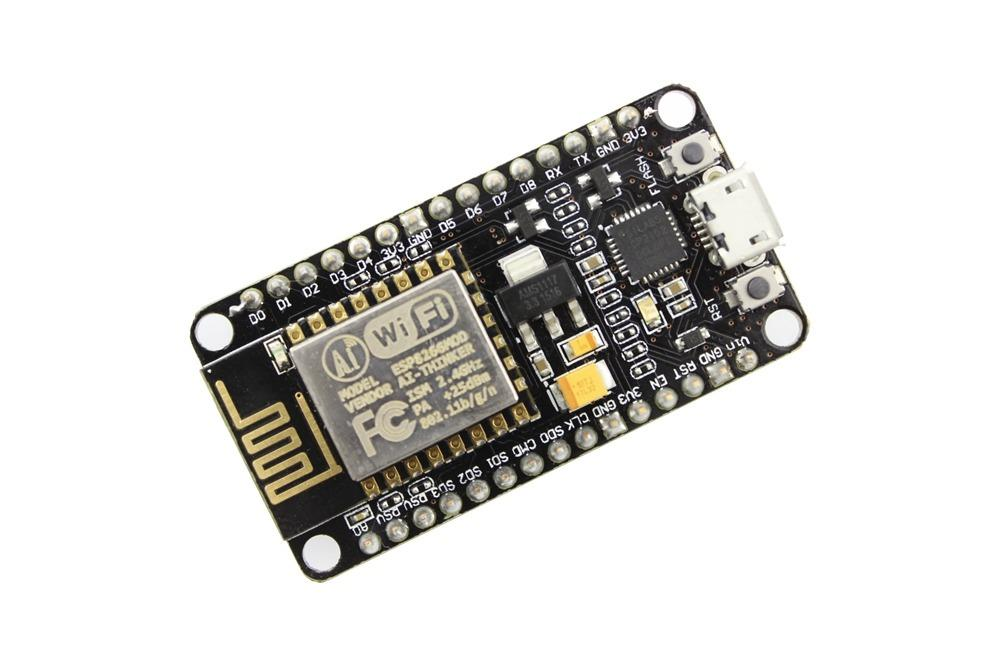
\includegraphics[width=0.7\linewidth]{img/esp8266}
%	\caption{ESP 8266}{Fuente: {\cite{esp8266}}}
%	\label{fig:esp8266}
%	
%\end{figure}

Es un microcontrolador fabricado por Espressif Systems que tiene las siguientes caracter�sticas:

\begin{itemize}
	\item N�cleo Xtensa Tensilica L106 de 32 bit con velocidad de 80MHz.
	\item 16 GPIO (Se puede configurar entradas, salidas, UART).
	\item  Un pin de entrada anal�gica
	\item Una memoria flash de 4 MB y 32kB de memoria RAM .
	\item  Convertidor anal�gico/digital de 10bit.
	\item Conectividad con WI-FI, pudiendo establecer servidores TCP/IP, UDP.
	\item Compatibilidad con SPI, I2C, I2S.
	
\end{itemize}


El dispositivo tiene un precio que var�a entre los 4\$ y los 7\$ {\cite{esp8266}} y puede programarse en lenguaje Simba, Lua o C. 


\subsection{ESP 32}
%\begin{figure}[H]
%	\centering
%	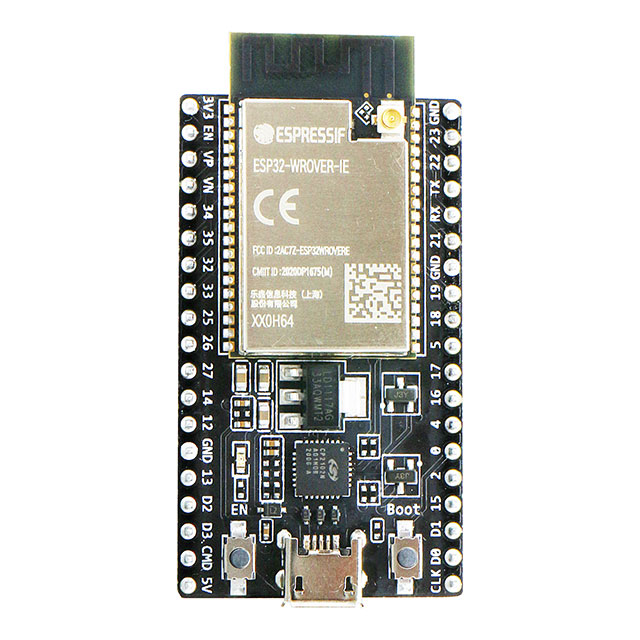
\includegraphics[width=0.7\linewidth]{img/Esp32}
%	\caption{Esp32}{{ \cite{rasberrypi}}}
%	\label{fig:esp32}
%	
%\end{figure}
El ESP32 fue creado por Espressif Systems emplea un microprocesador Tensilica Xtensa LX6 y posee las siguientes car�cteristicas:

\begin{itemize}
	\item Microprocesador32-bit Xtensa LX6 de doble n�cleo (o de un solo n�cleo), operando a 160 o 240 MHz y rindiendo hasta 600 DMIPS
	\item Veinticuatro pines GPIO, dieciocho pines anal�gicos ADC, sensores t�ctiles capacitivos, sensor de efecto Hall, amplificadores de bajo ruido, interfaz para tarjeta SD, Ethernet, SPI de alta velocidad, tres UART, I2S e I2C.
	\item Comunicaci�n Bluetooth, Wi-Fi  y BLE.
	\item Memoria RAM de 520 KiB SRAM.
	\item Velocidad de procesamiento entre 160 MHz y 240 MHz.
\end{itemize}

Este dispositivo tiene un costo entre 4\$ y 6\$ {\cite{esp32}} y puede programarse en lenguaje Python, Espressif IoT Development Framework, Zephyr Project, Mongoose OS, NuttX RTOS, C++.

\subsection{Selecci�n}


Los puntos a considerar para la selecci�n del microcontrolador se basaron en  las siguientes caracter�sticas:  velocidad de procesamiento, memoria RAM, que posea comunicaci�n por puerto serial y costo del dispositivo.

 Se necesita que la comunicaci�n entre el controlador y el emulador sea en tiempo real o con el m�nimo retardo, por esto, es importante saber cual es la velocidad de procesamiento del dispositivo.

La comunicaci�n entre la interfaz de emulaci�n y el controlador se realiza por puerto serial por este motivo se necesita un conector de puerto USB.

La memoria RAM es la que permite cargar todas las instrucciones que se mandan entre el dispositivo y el emulador.

Se estima que el costo del dispositivo sea accesible para los estudiantes que necesiten utilizar el programa y de este modo puedan implementar el dispositivo real.

Para seleccionar el dispositivo que mejor se ajusta a los requerimientos mencionados se utiliz� la tabla \ref{tabla:comparacion}.

\begin{table}[H]
	\caption{Comparaci�n de los dispositivos microcontroladores.}
	\setlength{\tabcolsep}{4pt} % default value: 6pt
	%% \centering % not needed since "tabularx" occupies full width of text block
	\begin{tabularx}{\textwidth}{@{} |Y|Y|Y|Y|Y| @{}}
		\hline
		\textbf{Dispositivo Microcontrolador} & 
		\textbf{Costo del dispositivo (En d�lares americanos)} & 
		\textbf{Velocidad de procesamiento} & 
		\textbf{Memoria RAM} & 
		\textbf{Puerto Serial}  \\
		
		\hline
		\textbf{Dispositivo ideal}
		& Menor posible \$
		& Mayor posible
		& Mayor posible
		& S� \\
		\hline
		
		\textbf{Arduino Ethernet(Est� descontinuado)}
		& Entre 45 y 55 \$
		& 16 MHz
		& 2KB
		& S� \\
		
		\hline
		\textbf{ESP8266}
		& Entre 4 y 7 \$		
		& 80MHz 
		& 32Kb
		& S�
		\\
		
	
	\hline
	
		\textbf{ESP32}
		& Entre 4 y 6\$
		& Entre 160 MHz y 240 MHz
		& 520 KiB SRAM
		& S�
		\\	
		\hline
	\end{tabularx}
\label{tabla:comparacion}
\end{table}

Se descart� el Arduino Ethernet ya que este dispositivo est� descontinuado. La elecci�n qued� entre el ESP8266 y el ESP32. 

El ESP8266 presenta una desventaja ya que solo posee un n�cleo, por este motivo se escogi� el ESP32 ya que cumple con tener un precio accesible, una velocidad de procesamiento y una memoria RAM suficientes para almacenar de manera correcta los datos del sistema de segundo orden.


 
